\section{Loi de Coulomb}

    \subsection{Champ électrostatique créé par une charge ponctuelle}

        On considère le système de deux particules chargées donné à la Figure~\ref{fig:champ_electrostatique_charge_ponctuelle}.

        \begin{figure}
            \centering
            \tikzsetnextfilename{champ_electrostatique_charge_ponctuelle}
            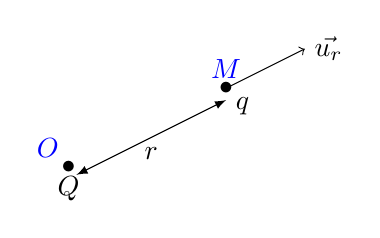
\begin{tikzpicture}[scale=1]  
                % \helpgrid{3}{3}
                \node at (0,0) {$\bullet$};
                \node[text=blue] at (0,0) [above left] {$O$};
                \node at (0,0) [below] {$Q$};

                \node at (2,1) {$\bullet$};
                \node[text=blue] at (2,1) [above] {$M$};
                \node at (2,1) [below right] {$q$};
                \draw[->] (2,1)--++(1,0.5) node [right] {$\vec{u_r}$};
                \draw[latex-latex] (0.1,-0.1) -- (2,0.85) node [below,midway] {$r$};
            \end{tikzpicture}
            \caption{Champ électrostatique créé par une charge ponctuelle.}    
            \label{fig:champ_electrostatique_charge_ponctuelle}
        \end{figure}

        On a 
        \begin{equation*}
            \boxed{
                \vec{F}_{Q\to q}=\frac{Qq}{4\pi\varepsilon_{0}r^{2}}\vec{u_r}.
            }
        \end{equation*}

        $\varepsilon_0$ est la permittivité électrique absolue du vide, avec $\varepsilon_{0}\mu_{0}c^{2}=1$ et 
        \begin{equation*}
            \boxed{
                c\approx 3.10^{8}~\si{\metre\per\second},\quad\mu_{0}\coloneqq 4\pi.10^{-7}~\si{\henry\per\metre},\quad \varepsilon_{0}\approx8.8.10^{-12}~\si{\farad\per\metre}.
            }
        \end{equation*}

        \paragraph{Champ électrostatique}

            On a une interaction à distance. Notamment,
            \begin{equation*}
                \vec{F}_{Q\to q}=q\vec{E}(M),
            \end{equation*}
            avec $\vec{E}(M)$ indépendant de $q$. Ainsi,
            \begin{equation*}
                \boxed{
                    \vec{E}(M)=\frac{Q}{4\pi\varepsilon_{0}r^{2}}\vec{u_r}.
                }
            \end{equation*}
            C'est la Loi de Coulomb. On a $[\vec{E}]=\si{\volt\per\metre}$.

    \subsection{Principe de superposition}

        C'est une conséquence de la linéarité des équations de Maxwell. S'il y a $N$ particules de charge $Q_i$, alors le champ électrostatique créé au point $M$ sur la particule de charge $q$ est 
        \begin{equation*}
            \boxed{
                \vec{E}(M)=\sum_{i=1}^{N}\vec{E_i}(M)=\frac{1}{4\pi\varepsilon_{0}}\sum_{i=1}^{N}\frac{Q_i}{r_i^{2}}\vec{u_{r_i}}.
            }
        \end{equation*}

    \subsection{Ordres de grandeur}

        \paragraph{Champ électrostatique de l'atome d'hydrogène}

            L'électron autour du noyau de l'atome d'hydrogène est à une distance $a_0=53~\si{\pico\metre}$ du noyau (rayon de Bohr). On a 
            \begin{equation*}
                \vec{F}=-q\vec{E},
            \end{equation*}
            avec
            \begin{equation*}
                E_{\text{proton}}=\frac{e}{4\pi\varepsilon_{0}a_{0}^{2}}\approx5.10^{11}~\si{\volt\per\metre}.
            \end{equation*}
            Notons que le rapport entre la force de gravitation et la force électrostatique exercée sur l'électron est 
            \begin{equation*}
                \frac{\left\lVert\vec{F}_{\text{gravitation}}^{p\to e}\right\rVert}{\left\lVert\vec{F}_{\text{es}}^{p\to e}\right\rVert}=\frac{\mathcal{G}m_p m_e}{\frac{e^{2}}{4\pi\varepsilon_{0}}}\approx 4.10^{-40}.
            \end{equation*}

        \paragraph{Champ disruptif de l'air}

            On a $E\sim 10^{6}~\si{\volt\per\metre}$.

        \paragraph{Échelle macroscopique}

            La batterie d'un téléphone portable crée un champ électrostatique est
            \begin{equation*}
                E\approx \frac{V}{d}\approx \frac{\text{qq } V}{\text{qq } \si{\centi\metre}}\approx10^{2}~\si{\volt\per\metre}.
            \end{equation*}